\documentclass[a4paper]{article}
\usepackage{geometry}
\usepackage{graphicx}
\usepackage{hyperref} 
\usepackage{booktabs}
\usepackage{amsmath}
\geometry{a4paper} 
\usepackage{subfig}

\usepackage[
        backend=biber,
        style=numeric,
        sorting=nyt,
    ]{biblatex} % looks like ieee
\addbibresource{references.bib}

% \usepackage{PRIMEarxiv}
% \usepackage[utf8]{inputenc} % allow utf-8 input
% \usepackage[T1]{fontenc}    % use 8-bit T1 fonts

% \fancyhead[LO]{Running Title for Header}

\renewcommand{\familydefault}{\sfdefault}

\begin{document}
% custom title page
\begin{titlepage}
  \begin{center}

    \vspace*{1cm}

    \textbf{\LARGE
    Understanding and evaluating data drift in computer vision from edge computing perspective
    }

    \vspace{1.5cm}

    % Author and Supervisor information
    \begin{center}
      \textbf{Janusz Jakub Wilczek} (Author) \\
      IT University of Copenhagen \\
      \textit{jawi@itu.dk} \\
      \vspace{0.5cm}  % Add vertical space between author and supervisors
      \textbf{Supervisors:} \\
      \begin{tabular}{@{}l@{}}
        Pinar Tözün IT University of Copenhagen, \textit{pito@itu.dk} \\
        Robert Bayer IT University of Copenhagen, \textit{roba@itu.dk}
      \end{tabular}
    \end{center}

    \vfill

    % degree
    A Thesis presented for the Degree of \\
    \textbf{Bachelor of Science in Data Science}

    \vspace{0.8cm}

    
\includegraphics{ITULogo}

    \vspace{0.8cm}


    \textbf{IT University of Copenhagen}\\
    Course Code: BIBAPRO1PE  \\
    \vspace{.5cm}
    May, 15th 2024

  \end{center}
\end{titlepage}

\newpage

% \tableofcontents
% \newpage

\begin{abstract} % (fold)
Concept drift (CD) detection in edge computing (EC) environments remains under-explored, with limited investigation into suitable techniques and their efficacy .Challenges such as inconsistent terminology complicate analysis, warranting a more stringent categorization approach. This study addresses this gap by examining CD detection methods in computer vision (CV) from EC perspective. However, due to incomplete experiments, further exploration is needed. Preliminary experiments highlight the critical role of batch size in detection accuracy. Overall, this study underscores the necessity for comprehensive exploration and evaluation of CD detection methods within EC and CV.
\end{abstract} 

\section{Introduction}
\label{sec:introduction}

The Internet of Things (IoT) presents a unique environment where devices are constrained in terms of computational power and memory. Despite these limitations, these devices can generate vast amounts of data \cite{merenda_edge_2020}. However, cloud computing often fails to meet applications' needs due to factors such as "low throughput, high latency, bandwidth bottlenecks, data privacy, centralized vulnerabilities, and additional costs" \cite{hua_edge_2023}. A potential solution lies in performing calculations directly on the edge devices, known as edge computing (EC), despite their inherent limitations \cite{hua_edge_2023}. 

Various steps of the ML life cycle have been explored from an EC perspective, including training, deployment, and pre-processing \cite{khouas_training_2024}\cite{murshed_machine_2021}\cite{ghosh_edge-cloud_2021}. However, ensuring the long-term success of ML models necessitates monitoring their performance. Young \cite{young_empirical_2022} has demonstrated the declining performance of various model architectures over time, where a decline has been observed for each. This phenomenon is known as model degradation.

ML engineers employ various approaches to address degradation, one of which is Continuous ML training and evaluation \cite{kreuzberger_machine_2023}, which entails regular updates to the models alongside testing. However, in the context of IoT ML, additional workload and data requirements are a larger challenge than in a more standard setting. A possible way to reduce those expenses would be to investigate the reasons behind model degradation and find a solution there.

Given ML's limited ability to abstract rules \cite{johnston_abstract_2023} \cite{marcus_deep_2018}, ML models are overly reliant on the training data. Thus, their performance is sensitive to the differences between training and production data. Therefore, any series of methods that can detect those differences, which could be linked to model degradation, are desirable. This would achieve two goals: reducing data transfer (data does not need to be transferred to obtain labels) and optimizing retraining time frames (they could be executed only when data drift is detected).

There have been two prominent names to describe this phenomenon: Data Drift (DD) and Concept Drift (CD). Problematically, there is a lack of consensus regarding what those terms describe. Furthermore, a mathematical description is elusive. This leads to a natural problem, especially in computer vision (CV), where highly dimensional data leads to larger computational needs, pushing EC to the limit. Therefore, in this paper, I aim to answer"

\begin{itemize}
    \item RQ: What is performance of unsupervised detection methods in detecting drift in CV tasks, in an EC environment?
\end{itemize}

\section{Background} % (fold)
\label{sec:background}

\subsection{What are data and concept drifts?}

Depending on the study, the meaning of data and concept drift is explained to various levels of detail. Some provide mathematical expressions, while others offer a couple of examples illustrating what constitutes drift, and still others stick with a brief verbal definition. This variability leads to ambiguity. For instance, \cite{lu_learning_2018} survey on concept drift defines it as:
\begin{quote}
    Concept drift means that the statistical properties of the target variable, which the model is trying to predict, change over time in unforeseen ways
\end{quote}

Their definition originates from Widmer and Kubat's paper \cite{widmer_learning_1996} and stands as one of the earliest formulations of the problem. However, since then, numerous other definitions and interpretations have emerged. This proliferation poses several challenges. Firstly, it complicates the translation of research insights into new scenarios, as the same term can encapsulate divergent ideas. Secondly, the abundance of terms and detection techniques unnecessarily complicates the evaluation process, leading to potential misapplication of techniques originally devised for different contexts.

Bayram \cite{bayram_concept_2022} has recognized this problem and organized terminology into six mathematical expressions (Table \ref{CD_defs}). What can be noticed is that the concept drift term has been used to essentially describe any change between training and production data. This bears impact on detection techniques, as one cannot claim change in posterior probability when a detection method looks at joint distributions.

\begin{table}[]
    \centering
    \def\arraystretch{1.3}
    \begin{equation}
    \begin{array}{@{}lll@{}}
    \toprule
      & \multicolumn{2}{c@{}}{\text{Concept Drift definitions}} \\
    \cmidrule(l){2-3}
      1 & P_t(X,y) \neq P_{t+w}(X,y) & \\
      2 &  P_t(y|X) \neq P_{t+w}(y|X) \\
      3 &  P_t(y|X) = P_{t+w}(y|X) \text{ and } P_t(X) \neq P_{t+w}(X) \\
      4 &  P_t(y|X) \neq P_{t+w}(y|X) \text{ and } P_t(X) = P_{t+w}(X) \\
      5 &  P_t(X) \neq P_{t+w}(X)  \\ 
      6 &  P_t(y) \neq P_{t+w}(y)  \\
    \bottomrule
    \end{array}
    \end{equation}
    \caption{Concept Drift mathematical definitions. $t, w$ respectively signify a specific time point and the time window within which the test is conducted.}
    \label{CD_defs}
\end{table}

It is note-worthy that another name commonly used to describe the same concepts as captured in Table (1) is data drift (DD). This terminology is particularly prevalent in ML medical imaging studies \cite{soin_chexstray_2022}, \cite{oala_data_2023}. Some papers' terminology goes as far as defining DD as the group name for all the changes between training and production data, wherein concept drift is one of many subcategories \cite{kore_empirical_2024}.

Nonetheless, a large part of the most prominent surveys in the field use CD as the name for all specific drift cases \cite{gemaque_overview_2020}, \cite{lu_learning_2018}, \cite{bayram_concept_2022}, \cite{barros_overview_2019}, \cite{barros_large-scale_2018}, \cite{krawczyk_ensemble_2017}, \cite{iwashita_overview_2019}. Thus, from now on, I will exclusively use CD.

\textbf{\subsection{Types of concept drifts}}

As it stems from mathematical definitions, CD is not only described by the magnitude of a change but also its place in time. There appears to be unanimous consensus in the field regarding categorization regarding the velocity of change and cycles (see Table \ref{CC_types}). Although similarly to the definitions, different terms have been used to describe the same notions. The types are a) sudden, b) gradual, c) recurring, d) incremental \cite{bayram_concept_2022}, visualized in Figure \ref{CC_types}.

\begin{figure}
    \centering
    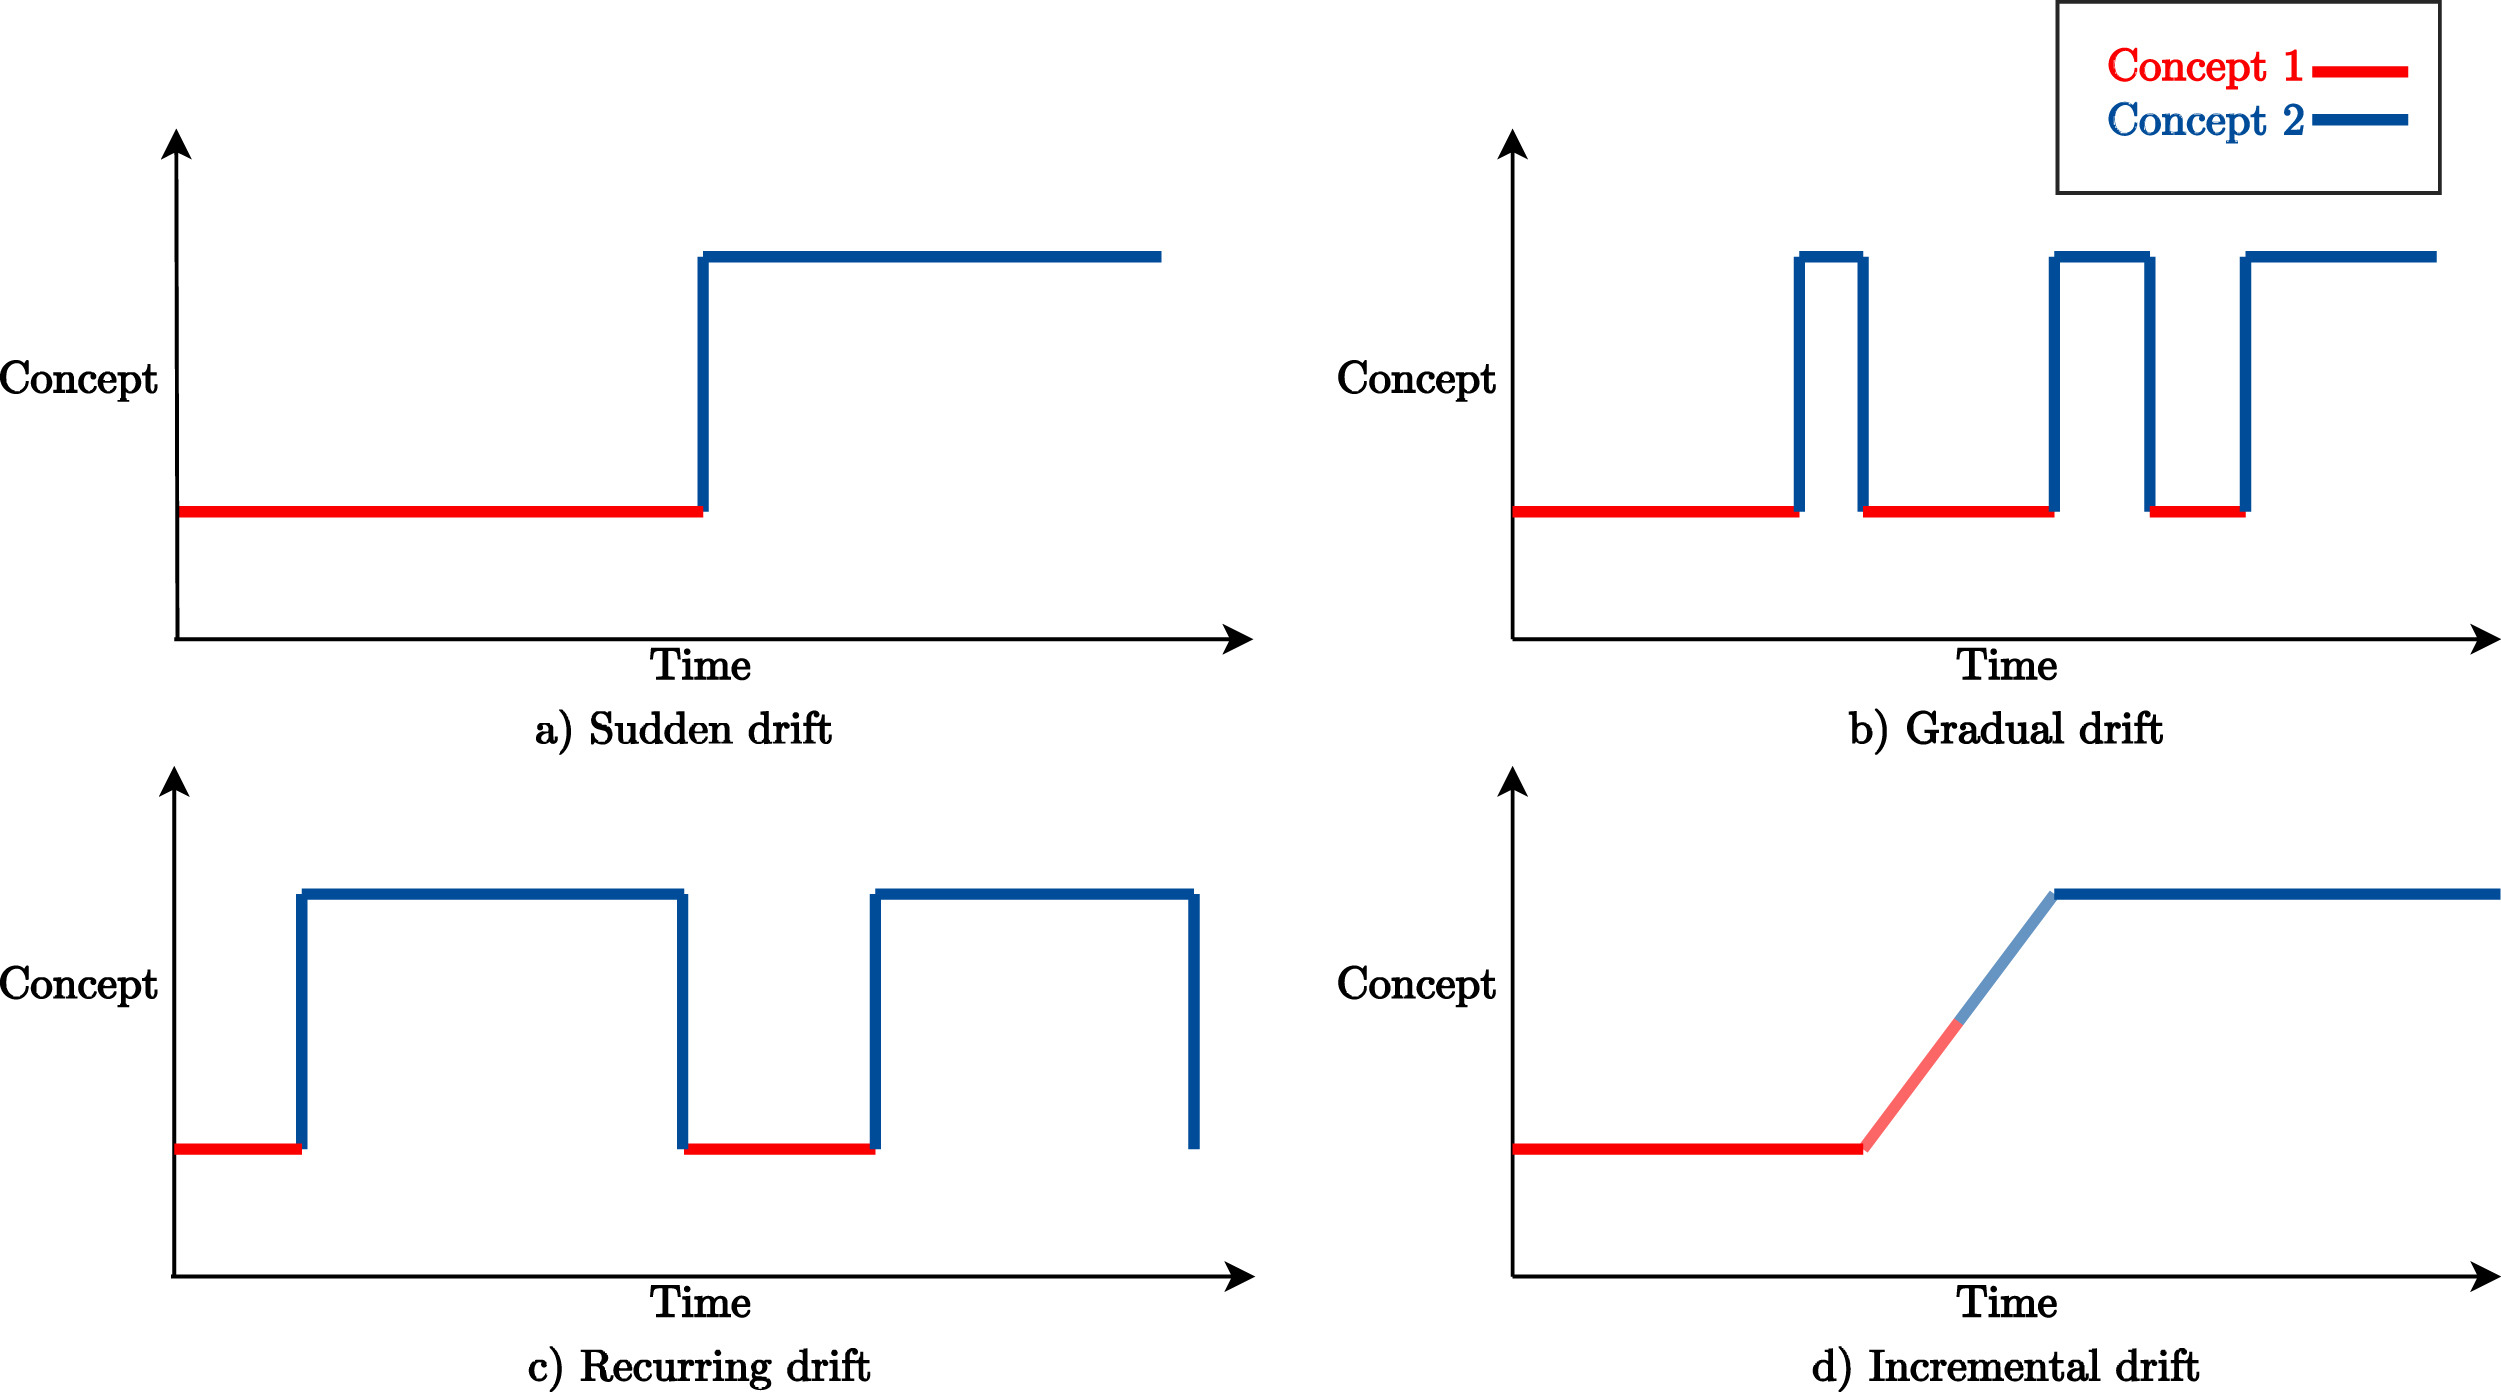
\includegraphics{images/CC types.jpg}
    \caption{Concept drift types. Figure source: \cite{bayram_concept_2022}}
    \label{CC_types}
\end{figure}


% \def\arraystretch{1.3}
% \begin{equation}
% \begin{array}{@{}lll@{}}
% \toprule
%   & \multicolumn{2}{c@{}}{\text{Concept Drift types regarding velocity of chnage}} \\
% \cmidrule(l){2-3}
%   1 Abrupt & sudden immiediate chnage\\
%   2 Gradual & incremental chnage \\
%   3 Recurring & \\
%   4 Incremental \\
% \bottomrule
% \end{array}
% \end{equation}

\subsection{What detection methods are available?}

There have been several distinct approaches to organize all concept drift detectors (CDD). \cite{bayram_concept_2022} organized performance-aware CDD according to the strategy used, e.g., ensemble learning. The issue with those methods from an EC perspective is that they require truth labels for the evaluation step, whose availability cannot always be assumed.

\cite{gemaque_overview_2020} created a conceptual overview of unsupervised CDDs, which do not require truth labels. In their taxonomy, models are first divided according to when and how detection is performed. The first distinction is made between online-based and batch-based methods, where the former checks each arriving data instance as they come, whereas the latter awaits until a batch is full.

Later, batch-based approaches can be divided based on whether they operate on a whole batch or a batch's subpart. In online-based methods, differentiation is made on how the reference window, i.e., the last known time before CD, is handled. Some CDDs have it fixed, whereas some slide it over time.

\subsection{What are examples of concept drift in computer vision?}

Notably, in the CD  field there has been a predominant interest in synthetic datasets. A benefit of this approach is a high customizability and control of the drift properties, so they thoroughly follow cases as described in table (1). Furthemore, even with a higher level of scrutiny with employmnt of mathematical expressions, it is challanging to claim a drift occurence in a real-world dataset, not to mention of what type and when \cite{cavalcante_fedd_2016}.

Many of common dataset generators are designed for classifications \cite{barros_overview_2019}, such as Sine \cite{baena-garcia_early_2006} and LED \cite{frias-blanco_online_2015}. On regression side, available datasets are limited \cite{bayram_concept_2022}, and they can be artificial too \cite{cavalcante_fedd_2016}. 

Regarding CV datasets, no generational approaches have been developed, so real world data must be used. As established before, this situation becomes difficult. One cannot easily claim a drift in a real world dataset, and intuitively it is more challenging to accurately capture it. A systematic review study on CD adaptation in video surveillance \cite{goncalves_concept_2024} collected 56 datasets. Importantly, none of them had annotations for CD. Therefore, it is worth exploring how researches have handled it CD investigations in the domain.

One of the examples is a compound set of CheXpert and PadChest datasets \cite{soin_chexstray_2022}, where data was combined and then divided according to the date of gathering. Those datasets are compound, i.e. contained both images and metadata. However, the study mostly focused on experimenting with metadata. Only one experiment had added lateral images, on which model was not trained on. \\

Another example is CXR dataset \cite{kore_empirical_2024} in where COVID-19 emergence from 2020 onwards is present, alongside a decrease with non COVID related cases. Suprem \cite{suprem_odin_2020} simulated CD in MNIST and CIFAR10 datasets. They 2 withhold classes for the training, which are later reintroduced in a production setting with a varying percentage of total classes they represent, between 0 to 50 percent. 

\subsection{Visualising CD}

% Having established some initial ground work into what CD is, it is worth to attempt visualise it. Figure 2 demonstrates a simple visualisation of all the figures. (Drop it as it will require a lot of effort to avoid an plagiarism)

% 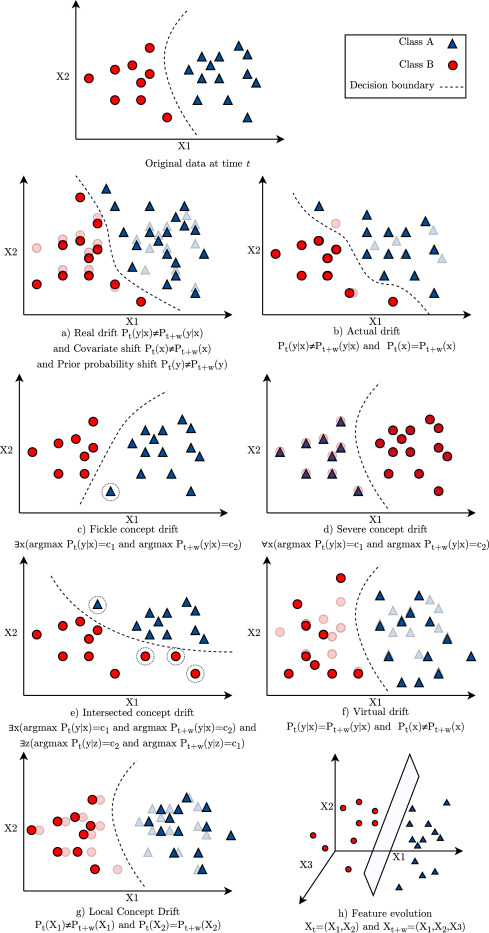
\includegraphics{images/Math visualised CD.jpg}
%\footnote{Figures 1 and 2 come from \cite{bayram_concept_2022}}

CD in CV presents a unique situation. Unlike regular tabular data, such as weather condition datasets with metrics like speed and temperature, for which humans are not capable of making factual assumptions about distributional changes that might have occurred just by looking at it. This holds especially true with datasets with a high number of features.

However, CV, by its nature, is different. People use their vision to discern whether images could have come from the same source. Figure \ref{Rot_img} shows the same car images from the CIFAR10 dataset: one original (a) and one rotated by 90 degrees (b). We can tell that the image is the same, just rotated. We would say that it still shows the same car. However, if we consider how the RGB values representing it shift in the data space, it can give us an intuition as to what drift can look like. ML classifiers mislabel rotated images \cite{cheng_learning_2016}, unless they have been incorporated in the training, for example, by data augmentation \cite{shorten_survey_2019}.

Importantly, rotational drift can have an impact on what a correct label should be. Figure \ref{Rot_5_img} contains a handwritten number 5 from the MNIST dataset, similarly as before in its unaltered state (a), and rotated (b). However, this time we would not necessarily intuitively claim that the rotated image still represents the digit 5. The interpretation depends on the design of the ML application \cite{shorten_survey_2019}. This might be a blind spot in unsupervised CDD methods.

\begin{figure}%
    \centering
    \subfloat[\centering CIFAR 10 original car image]{{
\includegraphics[width=5cm]{images/img_1301.png} }}%
    \qquad
    \subfloat[\centering Rotated car image by 90 degrees counter-clockwise]{{
\includegraphics[width=5cm]{images/img_1301_rot.png} }}%
    \caption{2 Figures side by side}%
    \label{Rot_img}%
\end{figure} 

\begin{figure}%
    \centering
    \subfloat[\centering MNIST no. 5 original image]{{
\includegraphics[width=5cm]{images/img_15_norm_5.png}}} %
    \qquad
    \subfloat[\centering Rotated no. 5 image by 90 degrees counter-clockwise]{{
\includegraphics[width=5cm]{images/img_15_rot_5.png}}}
    \caption{2 Figures side by side}%
    \label{Rot_5_img}%
\end{figure} 

\section{Experimental setting}

So far, research has focused on applying CD in various fields, evaluating CDD techniques, and conducting systematic reviews of the knowledge. Yet, no attention has been paid to evaluating those approaches from an EC perspective, where the workload impact of CDD approaches influences the applicability of a given method.

Therefore, in this paper, I investigate to what extent unsupervised CDD methods are able to detect drift while measuring their CPU and memory utilization.

To select methods for the experiments, I used techniques outlined by \cite{gemaque_overview_2020}. Out of that list, I highlighted whether I was able to find a publicly available implementation. This narrowed the list from the initial 17 instances to only 3. One technique was discarded as it was implemented in Java, whereas the other 2 were in Python. Since Python is an interpreted language whereas Java is compiled, it has an impact on CPU and memory utilization. Therefore, only Python implementations were used, namely the drift detection method based on active learning DDAL \cite{costa_drift_2018} and the Incremental Kolmogorov–Smirnov-based Drift Detector (IKS-bdd) \cite{dos_reis_fast_2016} \footnote{Since authors did not assign a name to the proposed technique, it was done by Gemaque \cite{gemaque_overview_2020} in their survey.}. 

\subsection{CDD: IKS-bdd and DDAL}

DDAL is a full batch-based approach, which calls for complete CD handling, from detection to re-training. However, I will focus on its ability to detect CD. This is achieved through the use of posterior probabilities from a model's output, compared to the user-defined hyperparameter called the uncertainty threshold. Each singular prediction is evaluated to determine whether it falls within confidence margins. This parameter governs the creation of virtual margins, set up as projections of hyperplanes. For instance, if the uncertainty threshold is set to 0.9, then for an object for which the maximum posterior value was lower than 0.9, it will be marked as significant. Once a batch is traversed, a density is calculated, which is the proportion of significant instances to the batch size. The minimum and maximum density values are stored and updated as the detection module evaluates incoming data. If the difference between the maximum and minimum densities exceeds another hyperparameter, named the drift threshold, drift is detected.

IKS-bdd is an online detector with a fixed reference window. It uses the Kolmogorov–Smirnov test to detect drift, which is applied to each feature space individually, avoiding performing multivariate tests and reducing computational complexity. It keeps two windows for each feature: a fixed reference window and a sliding one, which is being updated at each iteration. The IKS test is performed between these two windows at each iteration. If a test rejects the null hypothesis that data comes from the same distribution, then drift is signaled. 

\subsection{Data}
\label{sec:data}

In the experiments, adapted versions of the MNIST and CIFAR10 datasets are used, as shown in the image of \cite{suprem_odin_2020}. These datasets are a staple of CV, with images of low resolution, 28x28 pixels for MNIST and 32x32x3 pixels for CIFAR10. The reason being that neither DDAL nor IKS-bdd have been tested with image data. If they do not succeed in detecting drift on low-resolution images, then their ability to do so with higher resolution data is doubtful.

I apply dimensionality reduction to the CIFRAR10, converting it into a single channel, gray-scale pixels. I use PyTorch's function, which takes weighted sum from each channel.  

\subsection{Models for DDAL}

DDAL works with posterior probabilities, so a trained classifier is needed. I decided on using CNN for two reasons: 1) it has not been explored in either the DDAL proposing study or any of the surveys. 2) There were preliminary problems which are discussed later. The PyTorch library is used for the creation of classifiers.

The architecture used is presented in Table \ref{tab:cifar_cnn} and Table \ref{tab:mnist_cnn} for CIFAR10 \cite{noauthor_cifar-10_nodate} and MNIST respectively. Both models have been trained with the Adam optimizer \cite{noauthor_adam_nodate}, a learning rate of 0.0009, a batch size of 32, for up to 30 epochs with early stopping.

\subsection{Methodology}

Given the use of 2 different datasets, 2 different CDD techniques, 2 different CD types, with 2 different scenarios. CIFAR10 and MNIST are used, DDAL and IKS are CDD techniques of choice, abrupt and gradual CD types are simulated, and withhold and rotation drift scenarios are used.

The experiments can be divided into three sections: Fine-tuning DDAL hyper-parameters, evaluating accuracy of the CDD techniques, and measuring computational needs of those algorithms. 

Due to the lack of my intuition as to what are reasonable parameters, I run a series of runs across 
the whole hyperparameter space, i.e. from 0 to 1, with steps of 0.05, with additional finer steps within presumably optimal range, deduced from the initial random selection of hyper-parameter settings. Several batch sizes are tested too, withing range of 32 to 320, with each step being a multiple of 32. I run tests on each of the CDD cases, for both datasets, with an additional tests without the drift. Given EC setting, false positives can be detrimental, without providing increasing sensitivity. 

Having established what are reasonable parameters for the DDAL, a fair accuracy testing can be performed. Importantly, given 2 distinct CD scenarios, a separate evaluation approach is needed. In the abrupt setting, the drift should be detected as soon as it happens, and only once, as other detection would be false-positives. As to the gradual case, I design the drift that it begins to take place roughly at the middle batch of testing data, and steadily a new concept is introduced up to when it fully replaces the training one. Here I wish to see it highlight drift multiple times, since in the real application one cannot know to what degree the drift will take place.

Regarding computational needs, finally the experiments are run on an Raspberry Pi device, during of which CPU and memory data is being collected every second. 

\section{Results} % (fold)
\label{sec:results}

Fine-tuning results I analyse in the following manner, first I look at the runs without the drift. For the MNIST, it achieves no detections, which should be the case, for any tested batch size, for lambida's and theta's both being between 0.825 and 0.975. Notably, best runs did not detect any drift. For the CIFAR10 the results are less positive, In have found no pair of hyper-parameters that had no detections for the drift-less runs. The fewest number of false negatives was 4. Importantly, the best runs occur for similar values of theta and lambida, but only for the largest batch sizes of 288 and 320.

Secondly, I evaluate the specificity and sensitivity, with the values within those ranges, but with a drift introduced. There were two cases with a perfect detection for the MNIST abrupt withhold case, with the following parameters (Table: \ref{tab:best fine tune})

\begin{table}[]
    \centering
    \begin{tabular}{c|c|c|c|c}
        $\lambda$ & $\theta$ & Batch Size & Drift Started At & Drift Detected At \\
        \hline
        0.975 & 0.850 & 160 & 31 & 31 \\
        0.900 & 0.900 & 96 & 52 & 52 \\
    \end{tabular}
    \caption{Best hyper parameters for abrupt withhold class MNIST}
    \label{tab:best fine tune}
\end{table}

CIFAR10 runs with a drift performed highly regularly, yet disappointingly. Regardless of a whether a run had gradual or an abrupt drift, they all detected a drift at similar batch numbers, regardless of the hyper-parameters. I have not had many runs with small values of theta and lambida, but I would not expect them to perform much better given the experience with MNSIT. No run detects a drift at batch where it takes place for the abrupt, and I do not put faith in the true positive detections in the gradual scenarios. The only suggestion I can draw is that the best runs take place with a larger batch sizes.

Given all of the above, I settled on using the same set of hyper-parameters for both datasets and cases: \(\lambda = 0.975\), \(\theta = 0.850\), and a batch size of 160.

DDAL performance (Table: \ref{tab:Final results DDAL})  is varied and quite different from what I have expected given the fine tuning. However, it arguably trumps IKS's performance (Table: \ref{tab:Final results IKS}). 
\begin{table}[]
    \centering
    \begin{tabular}{c|c|c|c|c}
        \# & Dataset & Drift Case & Drift Started At & Drift Detected \\
        \hline
        0 & cifar & abrupt\_w-0 & 31.0 & [3, 16, 28, 44, 61] \\
        1 & cifar & gradual\_w-0 & 35.0 & [3] \\
        2 & cifar & rotate\_abrupt & 31.0 & [3, 16, 29, 39, 49, 59] \\
        3 & cifar & rotate\_gradual & 35.0 & [3, 15, 27, 41, 51, 59] \\
        4 & mnist & abrupt\_w-0 & 156.0 & [140] \\
        5 & mnist & clean\_test & NaN & [149] \\
        6 & mnist & gradual\_w-0 & 160.0 & [] \\
        7 & mnist & rotate\_abrupt & 156.0 & [118] \\
        8 & mnist & rotate\_gradual & 160.0 & [] \\
    \end{tabular}
    \caption{DDAL: Drift Detection Results Across Different Datasets and Experiment Setups
    W-0 is a withold of Class 0 scenario, rotate is a case with rotated images, and clean had no drift at all}
    \label{tab:Final results DDAL}
\end{table}

\begin{table}[]
    \centering
    \begin{tabular}{c|c|c|c|c}
        \# & Dataset & Drift Case & Drift Started At & Drift Detected \\
        \hline
        0 & cifar & abrupt\_w-0 & 156.0 & [] \\
        1 & cifar & gradual\_w-0 & 160.0 & [] \\
        2 & cifar & rotate\_abrupt & 156.0 & [] \\
        3 & cifar & rotate\_gradual & 160.0 & [] \\
        4 & mnist & abrupt\_w-0 & 156.0 & [] \\
        5 & mnist & clean\_test & NaN & [] \\
        6 & mnist & gradual\_w-0 & 160.0 & [] \\
        7 & mnist & rotate\_abrupt & 5000.0 & [] \\
        8 & mnist & rotate\_gradual & 160.0 & [] \\
    \end{tabular}
    \caption{IKS: Drift Detection Results Across Different Datasets and Experiment Setups
    W-0 is a withold of Class 0 scenario, rotate is a case with rotated images, and clean had no drift at all}
    \label{tab:Final results IKS}
\end{table}

Regarding computational needs, I experience that DDAL runs faster and drains less memory. However, I believe it is largely to unoptimised testing scenario, where many files of varied size, are saved, and IKS's setup makes it save more information. Quick and trivial optimisations, as introduction of batching resulted in significant improvements. Thus, I will come back to it and present more fair results during the defense.

\section{Discussion} % (fold)
\label{sec:Discussion}

My immediate reflection on the accuracy results is that a more through fine-tuning could. It appears that there exist no set of hyper-parameters that satisfies all the experimental scenarios, leading to a vastly divergent results among setups. Furthermore, a more detailed analysis of the results would be helpful. We can see, e.g. that DDAL (table: \ref {tab:Final results DDAL}) no. 5 detected drift in a clean setting, i.e. without any drift, although it had achieved to avoid so in some case in the fine-tuning. It might argue in favour of the DDAL's instability in detection, where in each run we could observe different results. 

Nonetheless, it is infinitely better than IKS. It failed to detect anything at any time-point. I have followed what has been described by \cite{dos_reis_fast_2016}, double checked it, yet it still failed to show any signs of viability in a CV task.

The past decade has witnessed a significant surge in scientific interest in machine learning (ML), with the absolute volume of published papers doubling to 483,000 in 2021 from just under 200,000 in 2010 (Our World in Data). Despite that, there are many challenges with CD.

Preliminary experiments with a decision tree have shown that it is a crucial step. The model was overfitted to the training space, which resulted in frequent high posterior probabilities (> 0.9) for each test sample. Similar situations might have taken place, as observed baseline accuracies have been much lower than the ones I observed during development. Initially, I was able to achieve accuracy scores of over 80\%, with a variance due to different hyperparameter choices and shuffling, on both datasets. However, in the end, I was reading partial accuracy scores of anything between 13\% to 60\%. It is an indication that either experimental data got corrupted, or artifacts had some issues. The accuracy score I mention here is a simple equal-weighted average since the datasets' class distributions were balanced.

There was a very limited amount of CDD techniques investigated. There are dozens of approaches, and using only 2 is not representative of them all. Furthermore, the lack of labels can be handled in semi-supervised ways, such as weak learning \cite{wang_ordisco_2021}.

Evaluating CDD requires more thoroughness than is considered in this paper. Firstly, there is a lack of a fair comparison. Some of the CDD in DDAL is carried out in C language, as large parts of PyTorch are written in it, whereas IKS-bdd is pure Python. Secondly, if a different machine was used for the experiments, it might have changed the results.

A substantial part of the CD field is drift adaptation, which has been entirely omitted in this paper. Some approaches, especially ensemble-based \cite{krawczyk_ensemble_2017}, provide interesting and promising solutions to both detection and adaptation. The use of ensemble also indicates that investigation from a model selection perspective can bring benefits in an EC setting.

The complexity and diversity of CD pose many problems when trying to analyze in EC. Few studies alongside conflicting nomenclature and terminology make this process more difficult than it would have been with consistent naming conventions.

Given the brought-up research, it is hard to evaluate whether the addition of a more stringent approach to categorizing CDD regarding mathematical formulations of what drift they deal with. However, it would mitigate the aforementioned aspect of inconsistent namings.

The choice of batch size was mostly arbitrary. \cite{baena-garcia_early_2006} has shown that its choice has a significant impact on DDAL's detection accuracy. Possibly, it is a trade-off between over-sensitivity and under-sensitivity, as batch size changes.

% section results (end)
\section{Conclusion}
\label{sub:Conclusion}

Rising interest in ML over years has brought many insights, including in regard to CD and CDD. Researchers have put effort into a creation of a systematical terminology and reviews, so to provide better overview and cope with term profeliation. Nonetheless, there are terminological issues, limited scope in CV and EC, and unreliable intuition what can be considered a drift. CDD techniques show promise for the low-resolution CV tasks, but are far from perfect. DDAL is dependent on the ML model it uses, a way in which it is trained, whereas IKS fails to the fullest degree. Regarding EC viability, it needs a further investigation. 

% bibliography
\newpage
% \bibliography{references} % Add references.bib file 
\printbibliography

\newpage
\section{Appendix} % (fold)
\label{sec:appendix}

\subsubsection{CNN architectures}

Tables \ref{tab:cifar_cnn} and \ref{tab:mnist_cnn} contain information on models structures. 

\begin{table}
\centering
\begin{tabular}{|p{3cm}|p{11cm}|} 
\hline
\textbf{Layer} & \textbf{Description} \\ \hline
Convolution (Input) & 1 channel, Output: 10 channels, Kernel Size: 5x5, Activation: ReLU, Pooling: Max Pooling (2x2) \\ \hline
Convolution & Input: 10 channels, Output: 20 channels, Kernel Size: 5x5, Activation: ReLU, Pooling: Max Pooling (2x2) with Dropout (before activation) \\ \hline
Flatten & $-$   \\ \hline
Fully Connected & Input: 320 features, Output: 50 features, Activation: ReLU \\ \hline
Dropout & Training only  \\ \hline
Fully Connected & Input: 50 features, Output: 10 features, Activation: Softmax \\ \hline
\end{tabular}
\caption{MNIST CNN Architecture}
\label{tab:mnist_cnn}  
\end{table}


\begin{table}
\centering
\begin{tabular}{|p{3cm}|p{11cm}|} 
\hline
\textbf{Layer} & \textbf{Description} \\ \hline
Convolution (Input) & 3 channels, Output: 32 channels, Kernel Size: 3x3, Padding: 1, Activation: ReLU \\ \hline
Pooling & Max Pooling (2x2, stride 2) \\ \hline
Convolution & Input: 32 channels, Output: 64 channels, Kernel Size: 3x3, Padding: 1, Activation: ReLU \\ \hline
Pooling & Max Pooling (2x2, stride 2) \\ \hline
Convolution & Input: 64 channels, Output: 128 channels, Kernel Size: 3x3, Padding: 1, Activation: ReLU \\ \hline
Pooling & Max Pooling (2x2, stride 2) \\ \hline
Flatten & $-$  \\ \hline
Dropout & Probability: 0.25 \\ \hline
Fully Connected & Input: 128 features, Output: 128 features, Activation: ReLU \\ \hline
Dropout & Probability: 0.5 \\ \hline
Fully Connected & Input: 128 features, Output: 10 features, Activation: Softmax \\ \hline
\end{tabular}
\caption{CIFAR10 CNN Architecture}
\label{tab:cifar_cnn}  
\end{table}

\subsection{Source code}

Main project code is avaiable at:
\href{https://github.com/ranUser01/TinyML}{GitHub}.
DDAL implementation:
\href{https://github.com/ranUser01/DDAL}{GitHub}.
IKS-bdd implementation:
\href{https://github.com/ranUser01/incremental_ks}{GitHub}.

\end{document}
